
%%%%%%%%%%%%%%%%%%%%%%%%%%%%%%%%%%%%%%%%%%%%%%%%%%%%%%%%%%%%%%%%%%%%%%
% Overleaf (WriteLaTeX) Example: Molecular Chemistry Presentation
%
% Source: http://www.overleaf.com
%
% In these slides we show how Overleaf can be used with standard 
% chemistry packages to easily create professional presentations.
% 
% Feel free to distribute this example, but please keep the referral
% to overleaf.com
% 
%%%%%%%%%%%%%%%%%%%%%%%%%%%%%%%%%%%%%%%%%%%%%%%%%%%%%%%%%%%%%%%%%%%%%%
% How to use Overleaf: 
%
% You edit the source code here on the left, and the preview on the
% right shows you the result within a few seconds.
%
% Bookmark this page and share the URL with your co-authors. They can
% edit at the same time!
%
% You can upload figures, bibliographies, custom classes and
% styles using the files menu.
%
% If you're new to LaTeX, the wikibook is a great place to start:
% http://en.wikibooks.org/wiki/LaTeX
%
%%%%%%%%%%%%%%%%%%%%%%%%%%%%%%%%%%%%%%%%%%%%%%%%%%%%%%%%%%%%%%%%%%%%%%

\documentclass[hyperref={colorlinks,citecolor=blue,linkcolor=blue,urlcolor=blue}]{beamer}

% For more themes, color themes and font themes, see:
% http://deic.uab.es/~iblanes/beamer_gallery/index_by_theme.html
%
\mode<presentation>
{
  \usetheme{Madrid}       % or try default, Darmstadt, Warsaw, ...
  \usecolortheme{default} % or try albatross, beaver, crane, ...
  \usefonttheme{serif}    % or try default, structurebold, ...
  \setbeamertemplate{navigation symbols}{}
  \setbeamertemplate{caption}[numbered]
} 

\usepackage[english]{babel}
\usepackage[utf8x]{inputenc}
\usepackage{chemfig}
\usepackage[version=3]{mhchem}
\usepackage{tikz}
\usetikzlibrary{plotmarks}
\usepackage{pgfplots}
\usepackage{lineno}
\usepackage{tikz}
\usepackage{xcolor}
\usepackage{subcaption}
\usepackage{pgf}  
\usepackage{svg}

\newlength\figureheight
\newlength\figurewidth
% \addtobeamertemplate{navigation symbols}{}{%
%     \usebeamerfont{footline}%
%     \usebeamercolor[fg]{footline}%
%     \hspace{5em}%
%     \insertframenumber/\inserttotalframenumber
% }

\setbeamertemplate{navigation symbols}{}
% \setbeamertemplate{footline}[frame number]{}
\setbeamertemplate{page number in head/foot}[totalframenumber]

% On Overleaf, these lines give you sharper preview images.
% You might want to `comment them out before you export, though.
\usepackage{pgfpages}
\pgfpagesuselayout{resize to}[%
  physical paper width=8in, physical paper height=6in]

% Here's where the presentation starts, with the info for the title slide
\title[]{Optimization test of Interconnected Natural Gas and Power Systems Using Mathematical Programs with Complementarity Constraints}
\author{Cristian Alejandro Blanco Martínez}
\institute{Universidad Tecnológica de Pereira \\ 
Grupo de investigación Automática}
\date{\today}

\begin{document}

\begin{frame}
  \titlepage
\end{frame}

% These three lines create an automatically generated table of contents.
\begin{frame}{Outline}
  \tableofcontents
\end{frame}

\section{Justification}
\begin{frame}{Relevance of natural gas}

Natural gas is an energy source that has acquired great relevance worldwide, and this can be attributed to two fundamental causes. 

\begin{itemize}
    \item It has been observed that a country's economic growth is closely related to its energy consumption.
    
    \item Natural gas emits less greenhouse gases compared to other fossil fuels, making it a favorable option for climate change mitigation.    
\end{itemize}

\end{frame}


\begin{frame}{Global and national context}

\begin{itemize}
    \item Global natural gas consumption in 2015 reached 124.24 trillion cubic feet, with a projected increase of 43\% by 2040, 75\% of which is associated with the industrial sector and power generation from thermal plants. 
    
    \item In the Colombian case, natural gas is a very important energy source because it is used in several sectors such as residential, commercial, industrial and thermal. It is especially in the latter where this fuel acquires greater relevance in dry seasons, since that is when the level of reservoirs is reduced and therefore also lowers the generation in hydroelectric plants. 

\end{itemize}

\end{frame}

\begin{frame}{Challenges in the Colombian energy system}
    
    Although most of the country's electricity demand is commonly supplied by hydroelectric power plants, this type of generation presents an important source of uncertainty in the energy system, since its effectiveness and generation capacity are directly linked to the country's weather and climate conditions.

\end{frame}

\begin{frame}{Problem statement}
\begin{figure}
    \centering
    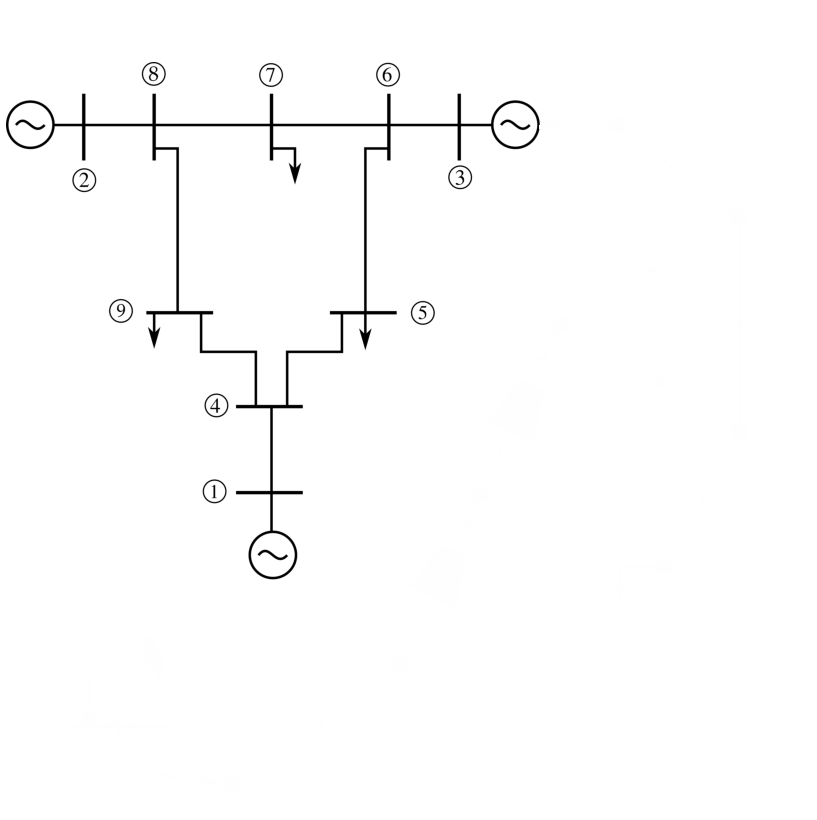
\includegraphics[scale=0.6]{figures/only_power.pdf}
    \caption{Caption}
    \label{fig:only_power}
\end{figure}
\end{frame}

\begin{frame}{Power system} 
\begin{figure}
    \centering
    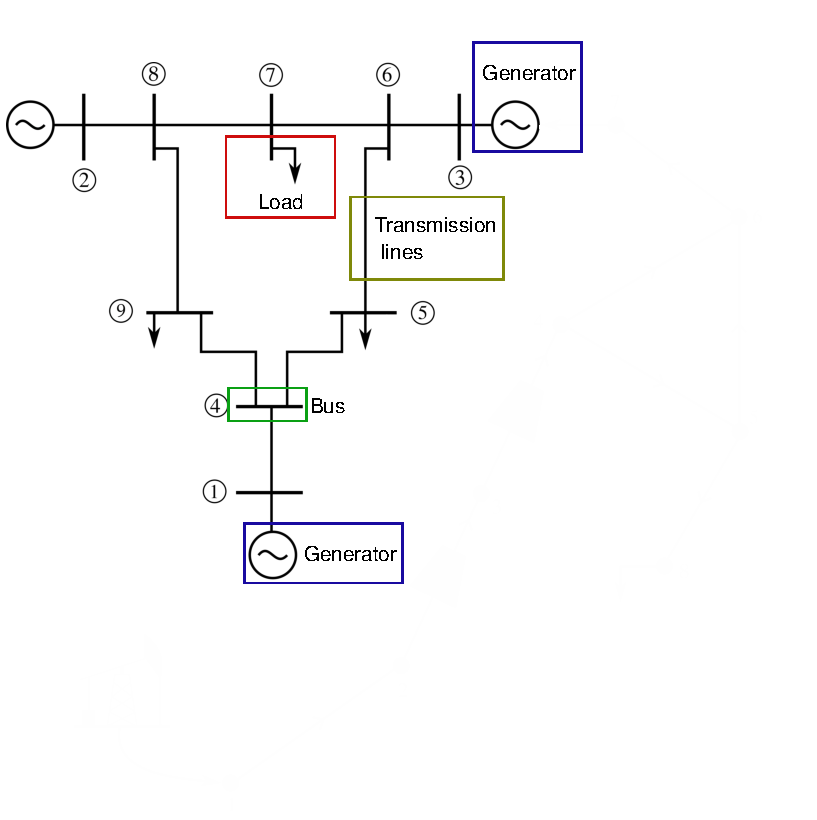
\includegraphics[scale=0.6]{figures/power_labels.pdf}
    \caption{Caption}
    \label{fig:power-labels}
\end{figure}
\end{frame}

\subsection{Gas system}
\begin{frame}{Interconnected system} 
\begin{figure}
    \centering
    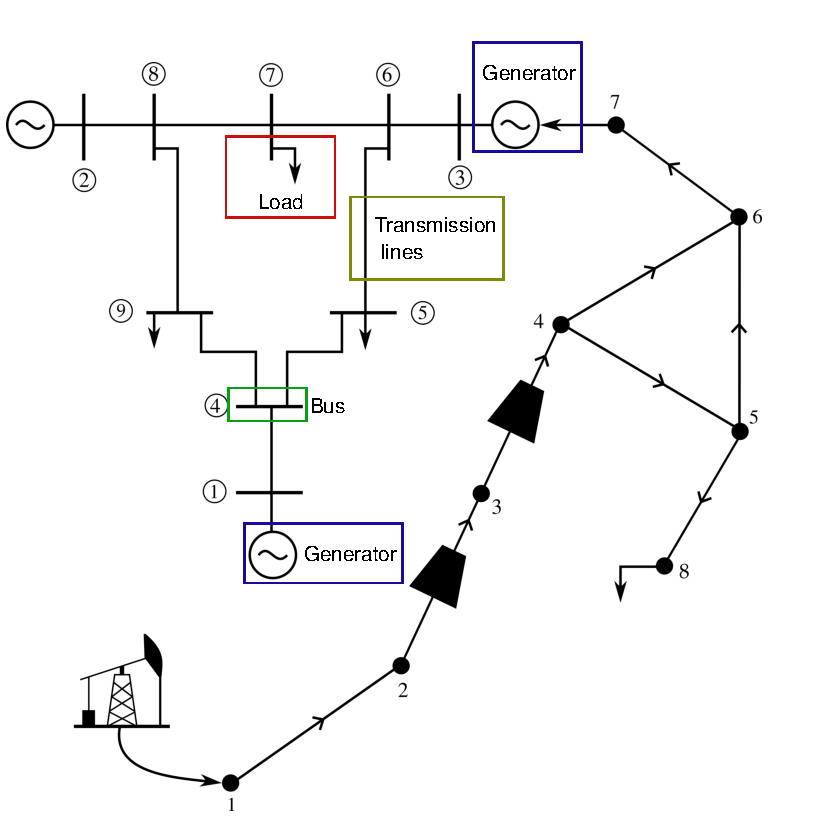
\includegraphics[scale=0.6]{figures/powe-gas.pdf}
    \caption{Caption}
    \label{fig:powe-gas}
\end{figure}
\end{frame}

\begin{frame}{Interconnected System} 
\begin{figure}
    \centering
    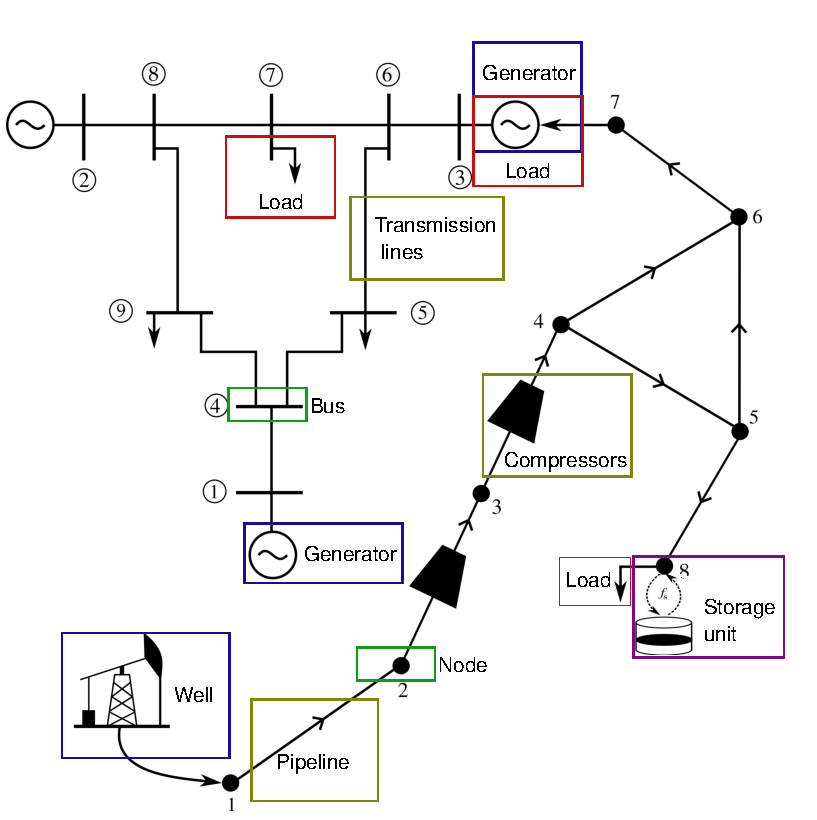
\includegraphics[scale=0.6]{figures/interconnected-full.pdf}
    \caption{Caption}
    \label{fig:interconneted-full}
\end{figure}
\end{frame}


\begin{frame}{Interconnected system - Definition}
A power-gas interconnected system is a hybrid infrastructure that integrates natural gas and power networks, enhancing overall system efficiency~\cite{Duan_Liu_Yang_2022}. Its key components include power generators, transmission lines, consumption buses, gas wells, pipelines, compressor stations, gas storage units, and consumption nodes. 
    
\end{frame}


\subsection{Model formulation}
\begin{frame}{Objective function}
\begin{columns}
\begin{column}{0.5\textwidth}
   \begin{center}
     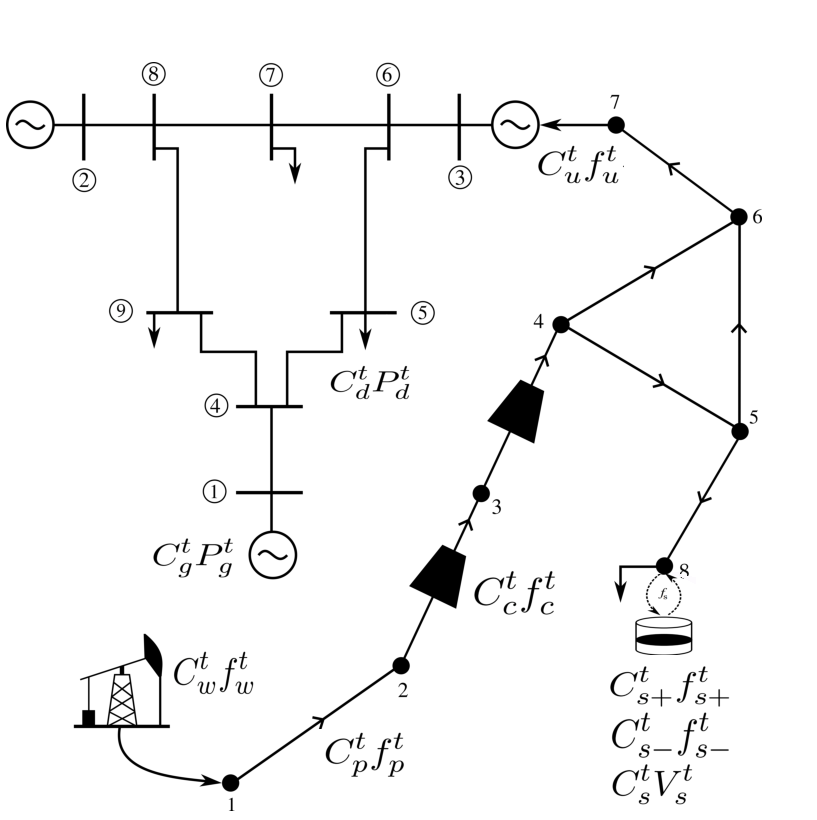
\includegraphics[width=1.1\textwidth]{figures/network_math_alternative.pdf}
     \end{center}
\end{column}
\begin{column}{0.5\textwidth}  %%<--- here
\begin{equation} \label{eq:obj_func_integrated}
\begin{split}
\min_{\mathcal{P}, \mathcal{F}} \quad  \sum_{g \in \mathcal{G}} C_{g}^t {P_{g}^t} + \sum_{d \in \mathcal{D}} C_{d}^t {P_{d}^t} +  \\ \sum_{w \in \mathcal{W}} C_{w}^t {f_{w}^t} +  \sum_{p \in \mathcal{P}} C_{p}^t {f_{p}^t}  + \\ \sum_{c \in \mathcal{C}} C_{c}^t {f_{c}^t} + \sum_{u \in \mathcal{U}} C_{u}^{t} {f_{u}^{t}} + \\ \quad \sum_{s \in \mathcal{S}} C_{s+}^{t} {f_{s+}^{t}}  + \sum_{s \in \mathcal{S}} C_{s-}^{t} {f_{s-}^{t}} + \\ \sum_{s \in \mathcal{S}} C_{s}^{t} {V_{s}^{t}}
\end{split}
\end{equation}
    
\end{column}
\end{columns}
\end{frame}

\begin{frame}{Power system constraints}

The constraints of the electrical system represent the technical limits of the different elements that compose it, as well as the physical laws that govern it. For certain applications, the DC model is sufficient~\cite{8468081}.

\begin{columns}
\begin{column}{0.24\textwidth}
% \begin{center}
\vspace{3pt}
    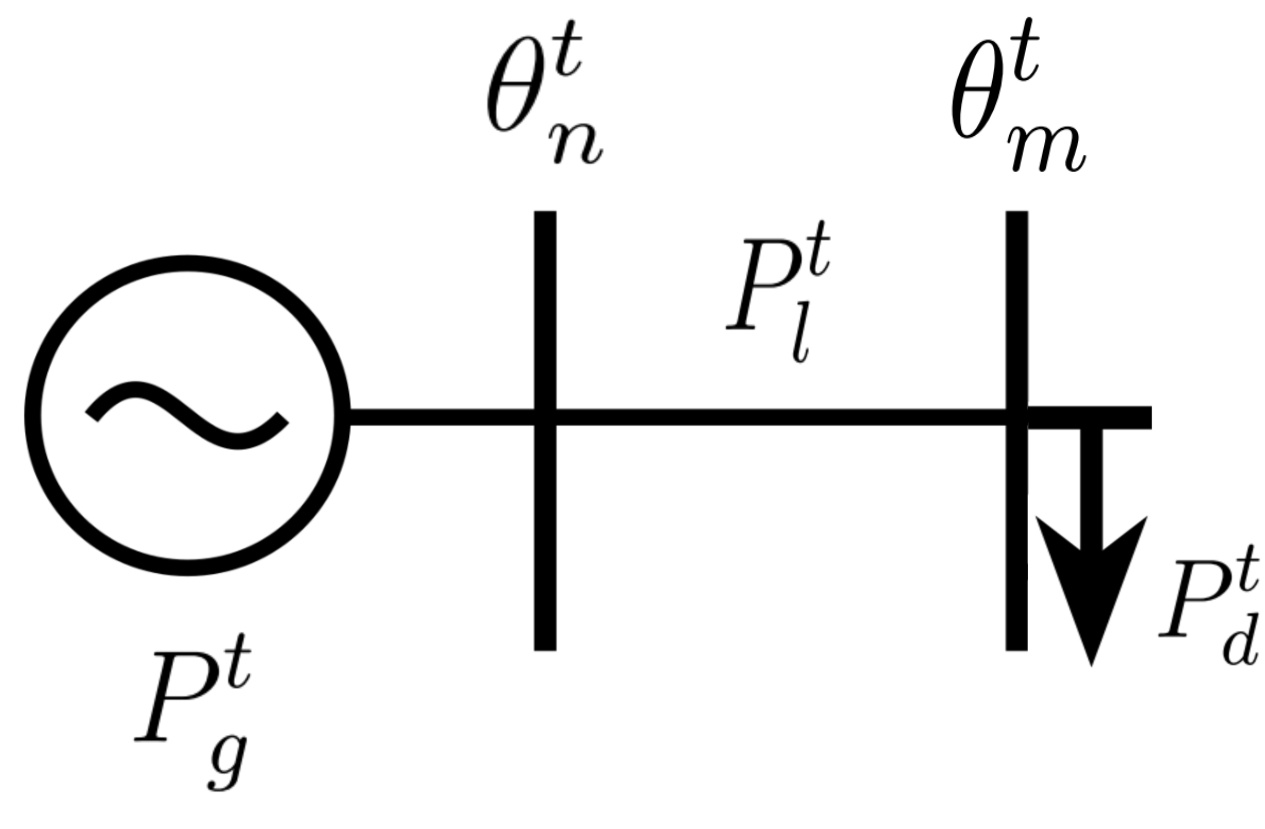
\includegraphics[width=1.4\textwidth]{figures/power_dummy_constraint.png}
% \end{center}
\end{column}
\begin{column}{0.8\textwidth}  %%<--- here

\begin{subequations}
\begin{alignat}{4}
    \underline{P_g^t} \leq P_{g}^t \leq \overline{P_g^t} &\quad \forall \ g \in \mathcal{G}, \label{eq:gen_limits} \\
    -\overline{P_l^t} \leq P_{l}^t \leq \overline{P_l^t} &\quad \forall \ l \in \mathcal{L}, \label{eq:line_limits} \\
    P_{l}^t = B_{nm}(\theta_n - \theta_{m}) &\quad \forall \ l = (n, m) \in \mathcal{L} , \label{eq:dc_power_flow} \\
    0 \leq P_{d}^t \leq \overline{P_{d}^t} &\quad \forall \ d \in \mathcal{D}, \label{eq:dem_limit_power} \\
    -\overline{\theta_{n}^t} \leq \theta_{m}^t \leq \overline{\theta_{n}^t} &\quad \forall \ n \in \mathcal{N}_P, \label{eq:voltage_angle_limits} \\
    \sum_{\substack{l\in \mathcal{L}_{n+}\\g=n}}{P_{l}^t + P_{g}^t} =  \sum_{\substack{l\in \mathcal{L}_{n-}\\d=n}} P_{l}^t + P_{d}^t &\quad \forall \ n \in \mathcal{N}_P \label{eq:power_balance} 
    % + \sum\limits_{n \in \mathcal{G}} P_{n}^t - \sum\limits_{n \in \mathcal{D}} P_{n}^t = 0 \quad \forall \ n,m \in \mathcal{N}_P \label{eq:power_balance} 
\end{alignat}
\end{subequations}

\end{column}
\end{columns}
\end{frame}

\begin{frame}{Interconnection constraints}
The second set of restrictions interconnects the natural gas and electric power systems through gas-fired power plants that generate electricity.  $f_{n}^t$ stands for the natural gas fuel consumption to generate a power $P_{n}^t$ at generator bus $n\in\mathcal{N}_I$, the heat-rate $\text{HR}_n$ defines the generator efficiency, and the set $\mathcal{N}_I=\mathcal{G}\cap\mathcal{U}$ holds all the units in the interconnected system belonging to both the power generator and gas demand sets.

\begin{figure}
    \centering
    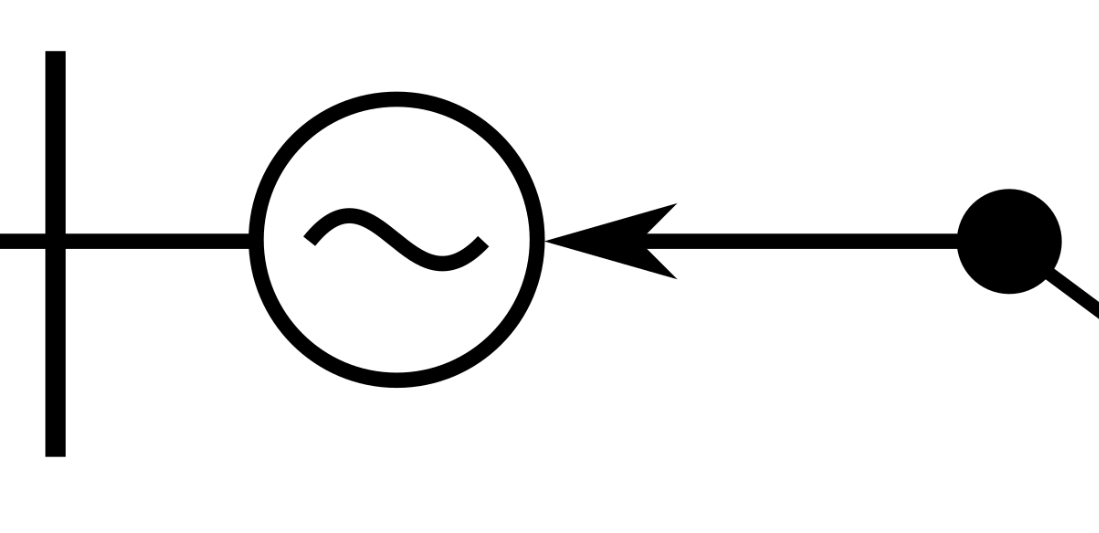
\includegraphics[width=0.4\textwidth]{figures/Interconection.png}
    \label{fig:enter-label}
\end{figure}

\begin{align}
    &f_{n}^t = P_{n}^t \cdot \text{HR}_n, \quad \forall \ n \in \mathcal{N}_I, \label{eq:gas_power_relation} 
\end{align}
\end{frame}


\begin{frame}{Gas system constraints}

This set of constraints ensures that wells, pipelines, nodal pressures, compressors, unsupplied demand and storage facilities operate within proper operating limits.~\cite{MPNG}.

\begin{columns}
\begin{column}{0.24\textwidth}
% \begin{center}
% \vspace{3pt}
    \includegraphics[width=1.5\textwidth]{figures/gas_dummy.png}
% \end{center}
\end{column}
\begin{column}{0.8\textwidth}  %%<--- here

 \begin{subequations}
\begin{alignat}{4}
    \underline{f_{w}^t} \leq f_{w}^t \leq \overline{f_{w}^t} &\quad \forall \ w \in \mathcal{W} \label{eq:well_limits} \\
    -\overline{f_{p}^t} \leq f_{p}^t \leq \overline{f_{p}^t} &\quad \forall \ p \in \mathcal{P} \label{eq:pipe_limits} \\
    \underline{\pi_{n}^t} \leq \pi_{n}^t \leq \overline{\pi_{n}^t} &\quad \forall \ n \in \mathcal{N}_f \label{eq:press_limit} \\
    \pi_{m}^t \leq \beta_{c}^t{\pi_{n}^t} &\quad \forall c=(n,m) \in \mathcal{C} \label{eq:comp_ratio} \\
    0 \leq f_{u}^{t} \leq \overline{f_{u}^{t}} &\quad \forall \ u \in \mathcal{U} \label{eq:dem_limit_gas} \\
    % \sum_{m:(m,n)\in\mathcal{A}}{f_{m}^t} = \sum_{m':(n,m')\in\mathcal{A}}{f_{m'}^t} &\quad \forall \ n \in \mathcal{N}_f \label{eq:gas_balance} \\
    0 \leq f_{s+}^t \leq V_{0s} - \underline{V_s} &\quad \forall \ s \in \mathcal{S} \label{eq:sto_limit1} \\ 
    0 \leq f_{s-}^t \leq \overline{V_s} - V_{0s} &\quad \forall \ s \in \mathcal{S} \label{eq:sto_limit2} \\ 
    V_{s}^t = V_{s}^{t-1} + f_{s-}^{t-1} - f_{s+}^{t-1} &\quad \forall \ s \in \mathcal{S} \label{eq:sto_time}\\
    % sgn(f_{p}^t)(f_{p}^t)^2 = K_{nm}((\pi_{n}^t)^2-(\pi_{m}^t)^2) &\quad \forall \ p =(n,m) \in\mathcal{P} \label{eq:weymouth_cons}
\end{alignat}
\end{subequations}
\end{column}
\end{columns}
\end{frame}






\section{Bibliography}
\begin{frame}[allowframebreaks]
        \frametitle{References}
        \bibliographystyle{apalike}
        \bibliography{biblio}
\end{frame}




\end{document}
